The goal of this task was to control the system around the optimal trajectory found in task 2 by means of Model Predictive control (hereafter referred as MPC).
\section{Problem setup}
In order to set up an MPC controller, the first step is to linearize around the desired trajectory. This way, we are able to use the \texttt{cvxpy} library to solve the problem quickly, by also taking into account possible path constraints on the input or the state.
We designed the function \texttt{linear\_ mpc} specifically to handle this task. At each time instant, we run the optimization problem on a time window of \texttt{$T_{mpc}$} and use the first input of the sequence. For plotting purposes we keep track of all the inputs we give to the system. 

\section{Parameters}
Even if we were able to tune the cost parameters $Q_{reg}$ and $R_{reg}$ as a degree of freedom, after running some experiments we found the same values we used in the optimization problem to be optimal. 
We implemented a random noise to be added. We tried to evaluate the system evolution for error on one individual component per experiments and the tracking was almost completely matching. However, for lack of space, these results won't be added in this report. 
We tried to evaluate the evolution of the system with the initial condition $x_0$ subject to a random error proportional to the maximum aplitude of each component, namely
\begin{equation}
 	x_{0,i}^{real}=x_{0,i}^{opt} \pm max_t(x_i^{opt})*p*randn, i \in 1,...,n
\end{equation}
with $p$ desired percentage, and $randn$ random number such that $-0.5<randn<0.5$. 
\section{Results}
Below are the plots for the results for $p$ varying from $10$ to $40$.

\begin{figure}[!h]
    \center
	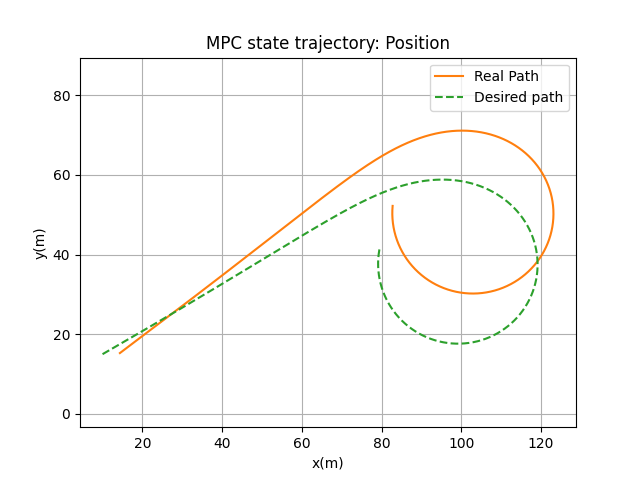
\includegraphics[height=70mm]{figs/_mpc_xy_5.png}	
	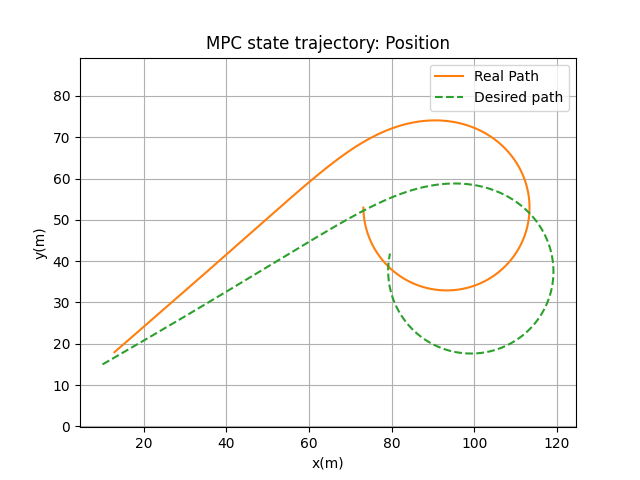
\includegraphics[height=70mm]{figs/_mpc_xy_10.png}	
    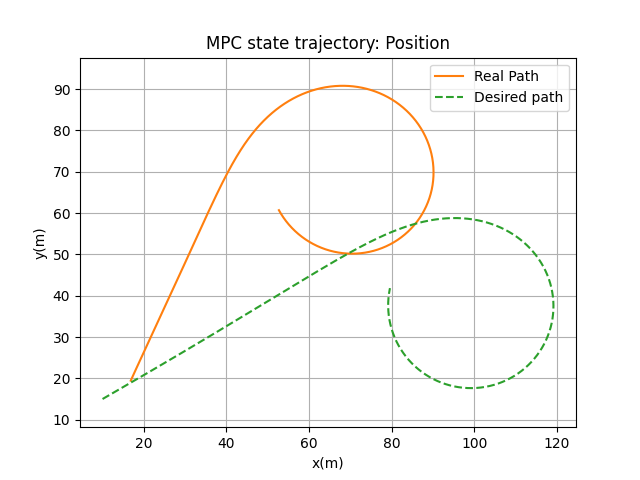
\includegraphics[height=70mm]{figs/_mpc_xy_20.png}	
	\caption{Tracked position trajectory with 5-10-20\% relative error on $x_0$}
\end{figure} 

\begin{figure}[!h]
    \center
	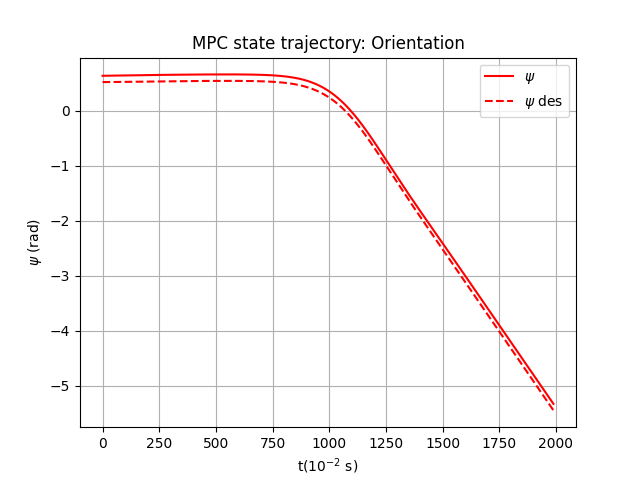
\includegraphics[height=70mm]{figs/_mpc_psi_5.png}	
	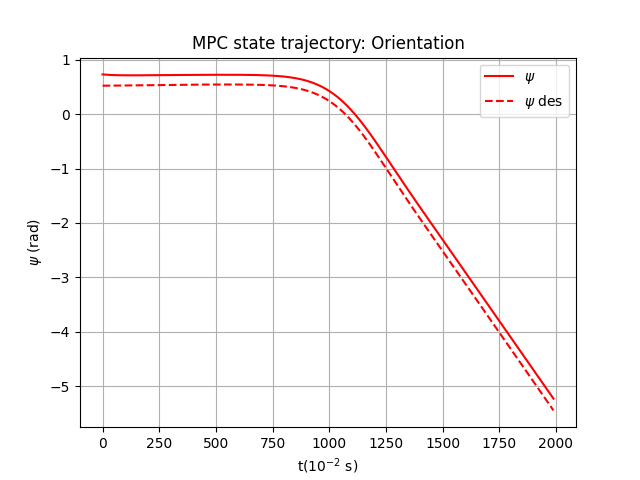
\includegraphics[height=70mm]{figs/_mpc_psi_10.png}	
    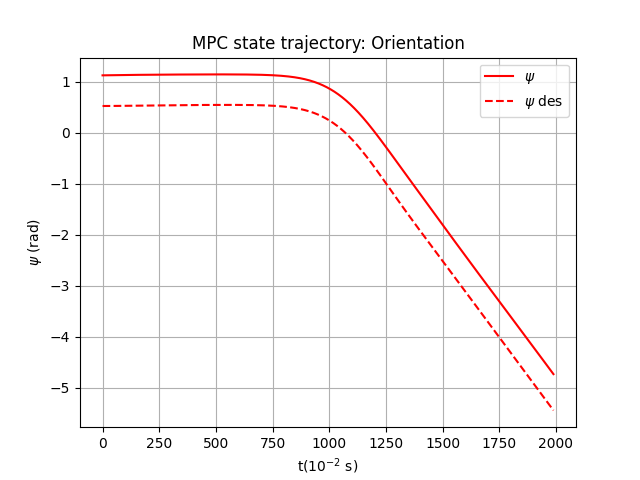
\includegraphics[height=70mm]{figs/_mpc_psi_20.png}	
	\caption{Tracked $\psi$ trajectory with 5-10-20\% relative error on $x_0$}
\end{figure} 

\begin{figure}[!h]
    \center
	\includegraphics[height=70mm]{figs/_mpc_V_5.png}	
	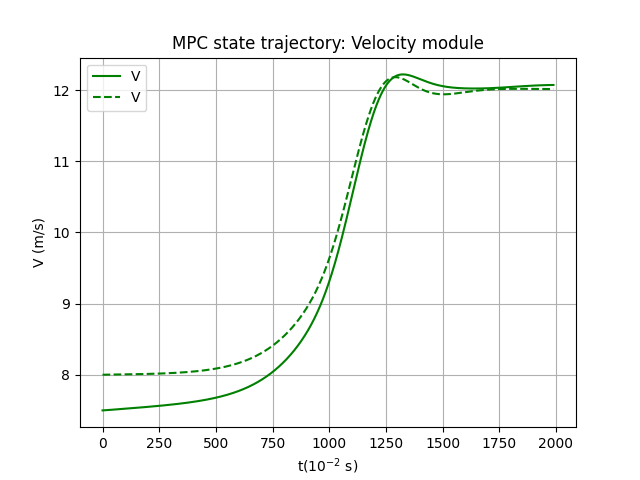
\includegraphics[height=70mm]{figs/_mpc_V_10.png}	
    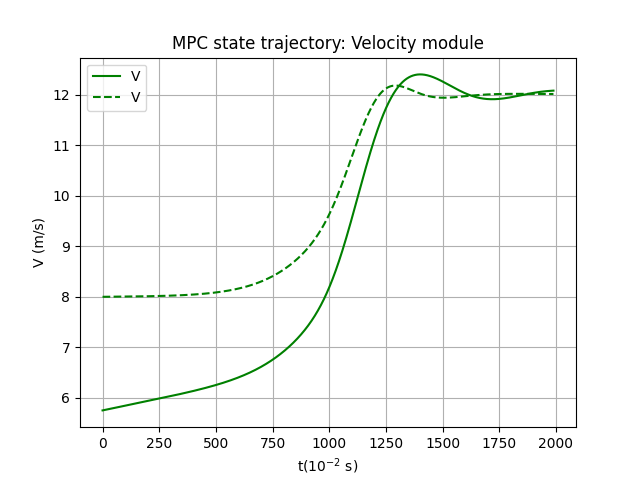
\includegraphics[height=70mm]{figs/_mpc_V_20.png}	
	\caption{Tracked $V$ trajectory with 5-10-20\% relative error on $x_0$}
\end{figure} 

\begin{figure}[!h]
    \center
	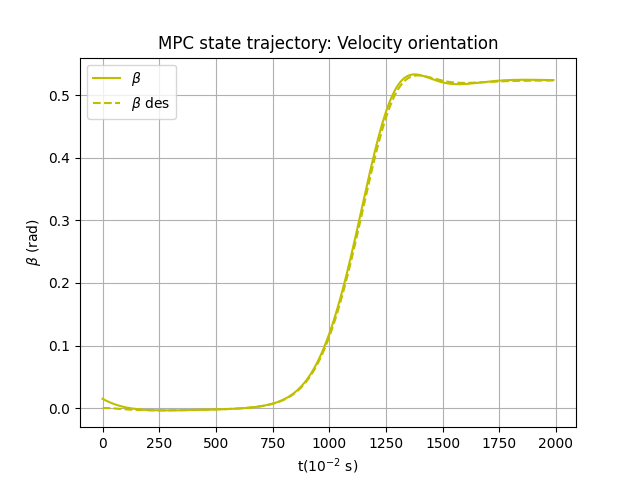
\includegraphics[height=70mm]{figs/_mpc_beta_5.png}	
	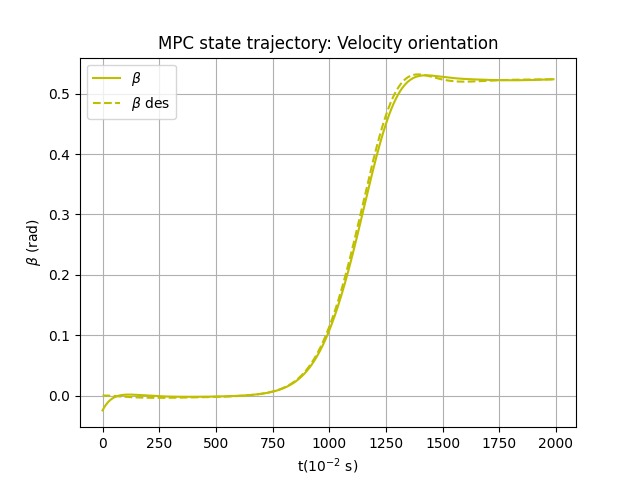
\includegraphics[height=70mm]{figs/_mpc_beta_10.png}	
    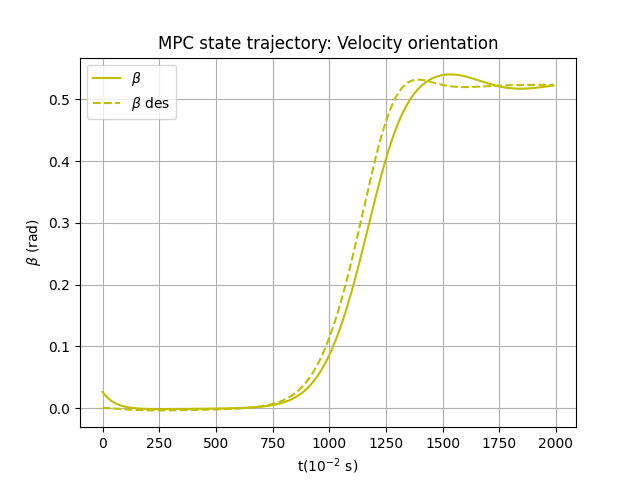
\includegraphics[height=70mm]{figs/_mpc_beta_20.png}	
	\caption{Tracked $\beta$ trajectory with 5-10-20\% relative error on $x_0$}
\end{figure} 

\begin{figure}[!h]
    \center
	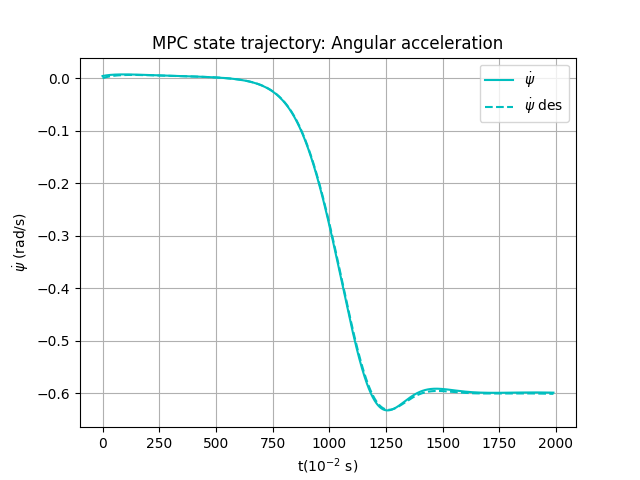
\includegraphics[height=70mm]{figs/_mpc_psidot_5.png}	
	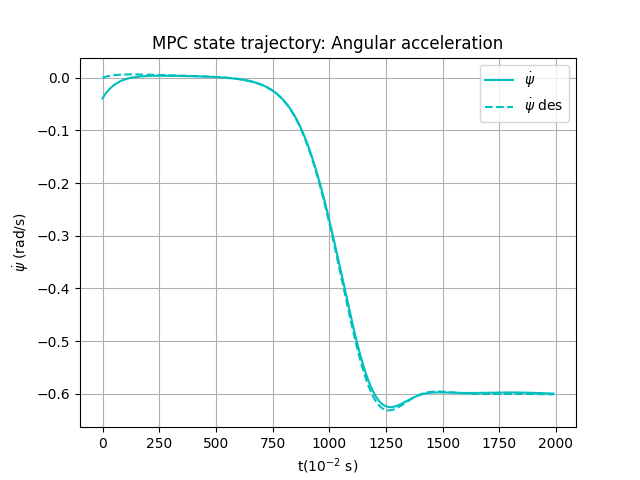
\includegraphics[height=70mm]{figs/_mpc_psidot_10.png}	
    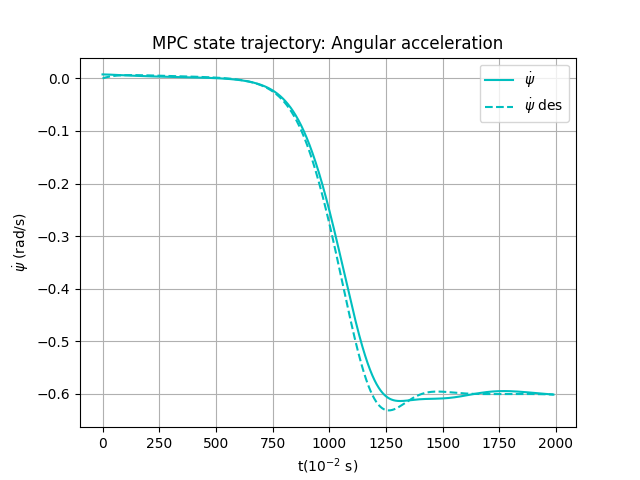
\includegraphics[height=70mm]{figs/_mpc_psidot_20.png}	
	\caption{Tracked $\dot{\psi}$ trajectory with 5-10-20\% relative error on $x_0$}
\end{figure} 

\begin{figure}[!h]
    \center
	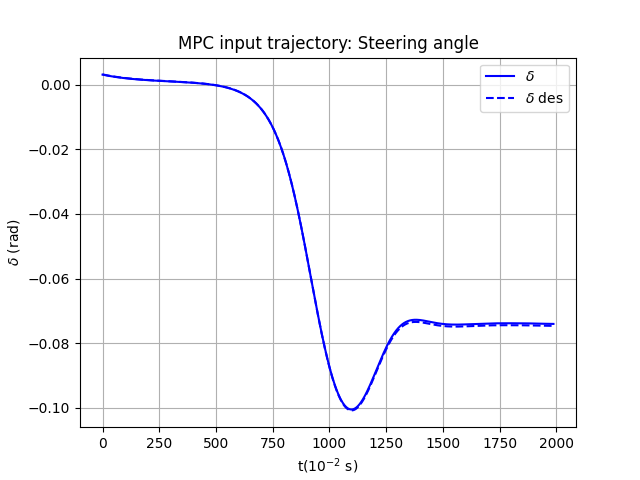
\includegraphics[height=70mm]{figs/_mpc_delta_5.png}	
	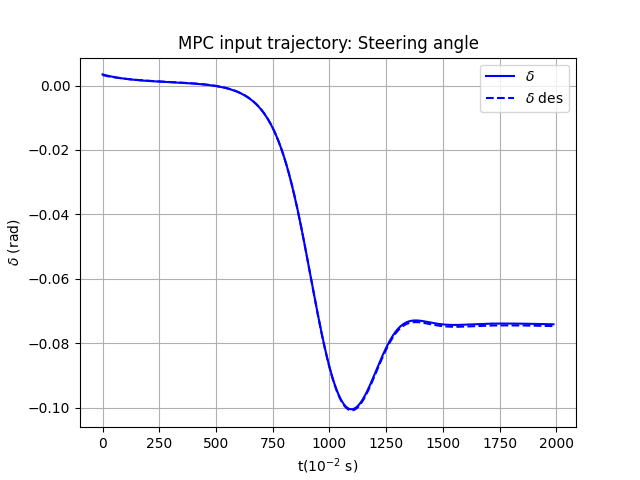
\includegraphics[height=70mm]{figs/_mpc_delta_10.png}	
    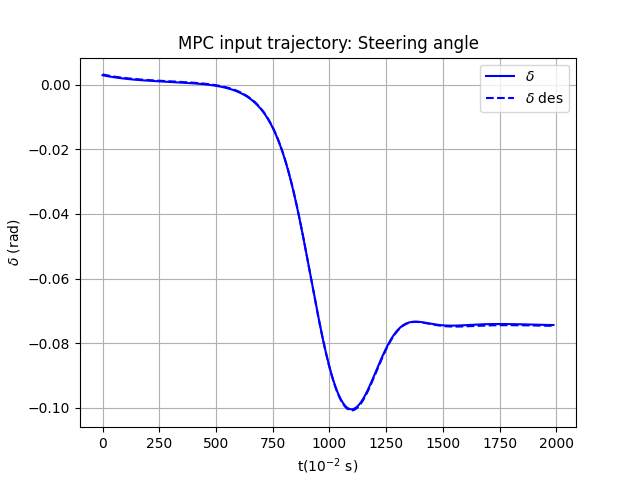
\includegraphics[height=70mm]{figs/_mpc_delta_20.png}	
	\caption{Tracked $\delta$ trajectory with 5-10-20\% relative error on $x_0$}
\end{figure} 

\begin{figure}[!h]
    \center
	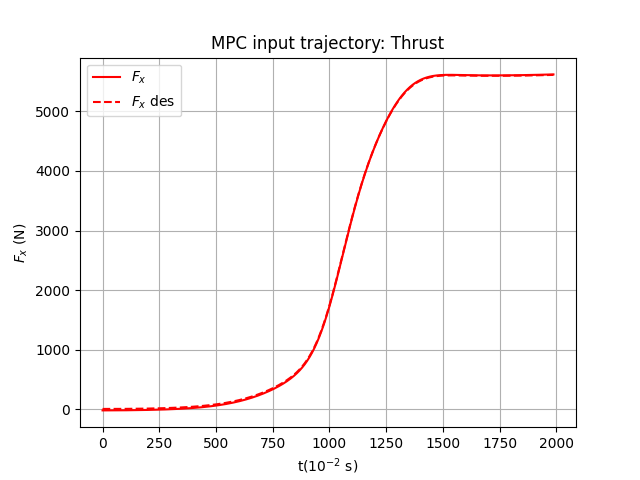
\includegraphics[height=70mm]{figs/_mpc_Fx_5.png}	
	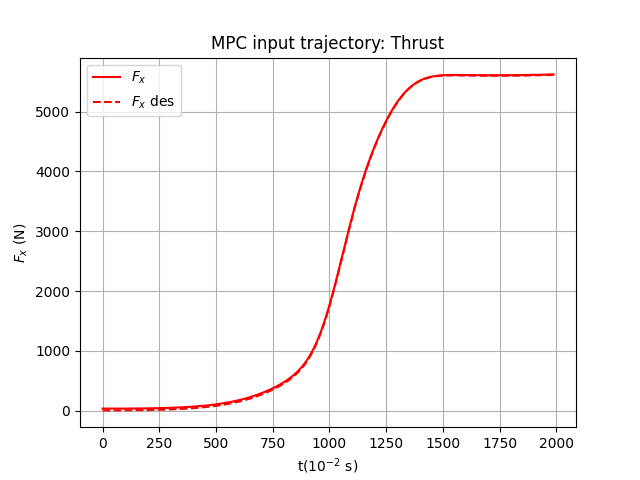
\includegraphics[height=70mm]{figs/_mpc_Fx_10.png}	
    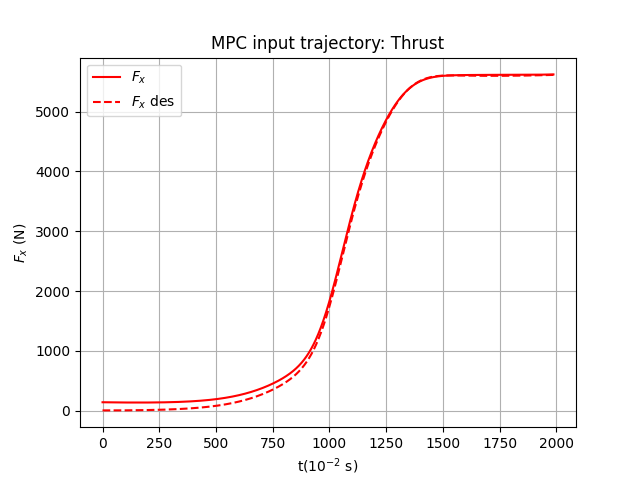
\includegraphics[height=70mm]{figs/_mpc_Fx_20.png}	
	\caption{Tracked $F_x$ trajectory with 5-10-20\% relative error on $x_0$}
\end{figure}

\section{Conclusions}
Altough the performances in tracking the velocities are good, even for a small error on the initial condition we reach considerable errors in the steady state values for the position and orientation variables. This is sensitively reduced when the error is on a single initial state component. We tried to address the problem by increasing the costs on the position variables and reducing the costs on the input but that had little to no result. We also tried with different time horizons $T_{mpc}$ and found 10 time instants to be the best trade off between efficiency for control and computational time. 
Overall, the MPC performances seem to be slightly worse than the LQR ones, but that is explainable via the fact that the LQR gains are computed by taking into account the whole trajectory for the system, while the MPC input takes into account only a small time window.